\documentclass[11pt, oneside]{article}  

\usepackage{style-3yp} %this is the .sty file
\usepackage{pdflscape}
\lfoot{Enzia Schnyder} %your name in the footer

\usepackage{float}
\usepackage{longtable}
\usepackage{gensymb} %degrees symbol
\usepackage [version=4] {mhchem}

%table
\usepackage{array}
\newcolumntype{L}{>{\centering\arraybackslash}m{2.5cm}}
\newcolumntype{J}{>{\centering\arraybackslash}m{4.1cm}}
\newcolumntype{M}{>{\centering\arraybackslash}m{5cm}}
\newcolumntype{N}{>{\centering\arraybackslash}m{3.5cm}}
\usepackage{multirow}

\begin{document}
\section{Gas Turbine}

\subsection{Introduction}\label{sec:intro}
A gas turbine system will be used in tandem with the SOFCs network to respond to sharp spikes in demand as gas turbines have a much shorter rise time so can be switched to full capacity quickly while the SOFC network slowly ramps up. It will burn the pre-cracked ammonia mixture in air to produce power. This section will first go through the design considerations and requirements of the turbine, followed by an explanation of the model used to find salient values and the final model results. The control problem of a step change in reference value for the turbine was also explored as well as an economic, environmental and safety analysis of the turbine system.

\subsection{Gas Turbine Design}
From analysis of the energy demand profile of Maui in section \ref{sec:plantscale}, it was concluded that the maximum turbine output required was 250MW. As the main purpose of the turbine is to respond quickly to sharp changes in demand, the most import design parameter is the rise time rather than efficiency. Other considerations are reliability, cost, safety, environmental impact and ease of operation/maintenance. The design parameters that can be chosen in optimising the turbine are equivalence ratio, turbine size, adiabatic flame temperature, cycle design, materials used and pressure ratio.\\The three different turbine configurations were considered were: %section label for 250MW power requirement
\begin {enumerate}
\item A single combined cycle 250MW turbine.
\item A single simple cycle 250MW turbine. 
\item Three parallel simple cycle 90MW turbines. 
\end {enumerate}
A multi-criteria analysis was performed to judge which configuration was the most suitable as shown in table 1 with each point being rated out of 5 with 5 being the most desirable outcome. 

\begin {table} [h]
\begin{center}
\caption{Multi-criteria analysis of the different turbine configurations} \label{tab:MCA} 
\begin{tabular}{ |c|c|c|c|c| }
 \hline
  Configuration & Rating & Single combined cycle & Single simple cycle & Multiple simple cycle\\ 
 \hline
  Cost & 4 & 2 & 5 & 5 \\ 
 \hline
  Efficiency & 3 & 5 & 3 & 3\\ 
 \hline
  Flexibility & 2 & 3 & 3 & 4\\
 \hline
  Rise time & 5 & 3 & 4 & 5\\
   \hline
   \multicolumn{2}{|c|}{Total}  & 44 & 55 & 62 \\
 \hline
\end{tabular}
\end{center}  
\end {table}
Weightings and scores were given as follows: 
\\\textbf{Cost - 4}: This is very important as the plant must be economically feasible to be built. However, the gas turbine is only a fraction of the total plant cost. Combined cycle plants are much more expensive than simple cycle at around 600-900 \$/kW compared to 300-350 \$/kW \cite{turbinecost}. For simple cycle turbines, there is a very small difference in cost/kW across the turbine sizes of interest so they both were scored at 5. Operation and maintenance costs are slightly lower for combined cycle and do not vary in cost/kW across single cycle turbines but these are less significant due to the low usage of the gas turbine in this plant. \cite{boyce} Therefore the combined cycle option was given a low score of 2 and the simple cycle options were given high scores of 5.
\\\textbf{Efficiency - 3}: Efficiency is important as it determines how much energy will need to be put into the turbine to achieve a given output, which determines the flow rate of ammonia required and factors heavily into operation costs. However, as most of the energy generated by the plant will come from the SOFCs, it is weighted less heavily . The gas turbine will also be used at peak demand time when electricity prices are high. Combined cycle systems are significantly more efficient than simple cycle at around 55\% compared to 40\% so option 1 was given a score of 5. For simple cycle turbines, 250MW turbines are only marginally more efficient than 90MW turbines (around 1\%). However, the parallel configuration of option 3 would allow the turbines being used to operate at full load (and maximum efficiency) more of the time so they were both given scores of 3.
\\\textbf{Flexibility - 2}: The turbine system will operate at a variable load so it must be flexible. It has a low weighting as variations in flexibility are relatively small across the three options. The large turbines are more limited due to their minimum operating loads (around 35\% for combined cycle and 45\% for simple cycle) \cite{boyce}. The small parallel turbines give greater flexibility as they do not all have to be used at a given time and can continue to be used at 66\% of full load under maintenance periods. The modular system also allows more turbines to be added or removed depending on long term changes in energy demand of Maui \cite{website:multipleunits}. %boyce citation is wrong!!
\\\textbf{Rise time - 5}: A fast rise time is essential as the main purpose of the turbine system is to provide power during large surges in demand. Combined cycle performs with the greatest rise time as the steam cycle heats up slowly. Simple cycle turbines have a much faster rise time, which decreases with size. Option 3 will have the fastest rise time as the 3 turbines will be able to ramp up in parallel \cite{website:multipleunits}. 
\\\textbf{Other factors}: Other factors such as environmental impact, safety and ease of operation were not included as there was a smaller difference in impact across the three options.\\
The analysis shows that option 3, three parallel 90MW turbines, was the most suitable for this project, although the margins were close and option 2 could also feasibly be used. Option 1 would be more suitable for a project with a greater weighting on efficiency (i.e. if the turbine was the sole power generator of the plant).

\subsection{Limitations of Ammonia as a Fuel \cite{verkamp}}
Ammonia provides many challenges as a combustible fuel. Its high ignition energy, high heat of vapourisation and low lower calorific value (LCV) mean that a lot of energy must be put into combustion. Additionally, it also has narrow flammability limits, limiting the range of equivalence ratios that can be used.  Different methods to mitigate this that were considered were:
\begin {enumerate}
\item Mixing hydrocarbons into the ammonia. - This would improve combustion properties but at the cost of a high negative environmental impact due to the carbon emissions and the impact of extracting and transporting natural gas to the plant. 
\item Burn a mixture of ammonia and hydrogen. - The burning properties of hydrogen are much better than ammonia. A precracker can be used to partially dissociate the ammonia into hydrogen and nitrogen so that a mixture of the three gases is run through the combustion chamber. As hydrogen is much easier to combust than ammonia, a dissociation ratio can be chosen to achieve combustion properties comparable to that of hydrocarbons. \cite{verkamp}
\item Oxygen enriched combustion of ammonia. - Oxygen enriched combustion is a common technique used to decrease the energy input needed to burn fuels, and it has been also shown to increase fuel consumption at equal stoichiometric ratios \cite{baskar}. By adding excess oxygen, which can be taken as a waste product from the electrolyser, the mass flow rate of the air will also decrease, improving cycle efficiency. 
\item Gas turbine modifications. - A standard gas turbine can be modified to burn ammonia, which would include using a higher input ignition energy and larger size to accommodate for decreased air flow rate due to the lower flame stability of ammonia. However, this would be very expensive in both capital and operating costs. \cite{} %CITE THIS
\end {enumerate}

It was decided to use methods 2 and 3 together to improve ammonia combustion. A precracker will be used to partially dissociate the ammonia coming from storage, which will be burnt in the combustion chamber with air and the waste oxygen from the electrolyser.

\subsubsection{Dissociation Ratio}
To find the appropriate dissociation ratio, the properties of ammonia and hydrogen were compared with conventional fuels diesel and gasoline as shown in table \ref{tab:burningproperties}.

\begin{table} [h]
\begin{center}
\caption{The burning properties of ammonia, hydrogen, diesel and gasoline \cite{garabedian}}\label{tab:burningproperties}
\begin{tabular}{ |c|c|L|L|L|L| }
 \hline
  Fuel & LCV (MJ/kg) \cite{website:spg} & Ignition energy (mJ) & Stoichiometric AFR by mass & Autoignition temperature (\degree F) & Flame speed (cm/s) \\ 
 \hline
  $NH_3$ & 18.6 & 9.0 & 0.1653 & 1200 & 33 \\ 
 \hline
$H_2$ & 120.1 & 0.18 & 0.0292 & 1170 & 300\\ 
 \hline
Diesel & 42.8 & 0.3 & 0.068 & 500 & 100\\
 \hline
 Gasoline & 42.5 & 0.3 & 0.068 & 800 & 100\\
 \hline
\end{tabular}
\end{center} 
\end{table}


A trade-off must be found between optimising burning properties and having too much hydrogen, which will lead to an unstable, rapid burning and high combustion temperatures. 

  \begin{figure} [h]
\centering
\begin{subfigure}{.5\textwidth}
  \centering
  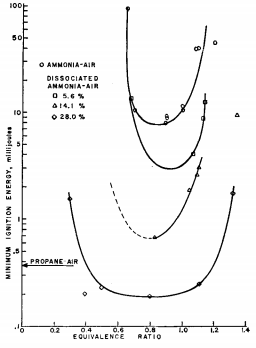
\includegraphics[width=0.9\linewidth]{./pictures/ignitionenergyNH3.png}
  \label{fig:mixproperties1}
\end{subfigure}%
\begin{subfigure}{.5\textwidth}
  \centering
  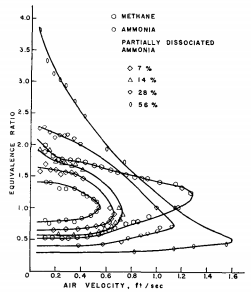
\includegraphics[width=0.9\linewidth]{./pictures/flamestabilityNH3.png}
  \label{fig:sub2}
\end{subfigure}
\caption{(a) The ignition energy and (b) flame-stability properties of methane-air, ammonia-air and partially dissociated ammonia-air \cite{verkamp}}
\label{fig:mixproperties2}
\end{figure} 

The figure \ref{fig:mixproperties2} suggests that 28\% dissociation still had a minimum ignition energy higher than that of propane-air (8mJ compared to 0.37mJ at a similar equivalence ratio), which suggests a higher dissociation is required. Li et. al. \cite{junLi} also showed that 54.5\% dissociation had a similar burning velocity to methane. We want the mixture to behave similarly to natural gas, which is composed of methane (93.9\%), ethane (4.2\%) and propane (0.3\%) \cite{website:uniongas}, so that no modifications need to be made to the turbine. Therefore a dissociation of 38\% will be used with dissociation reaction:

\begin{equation}
\ce{NH_3 -> 0.62 NH_3 + 0.19 N_2 + 0.57 H_2}
\end{equation}

Assuming that dry air is made of 79\% $N_2^*$ and 21\% $O_2$ where $N_2^*$ is used to represents all components of air other than oxygen the combustion reaction for one mole of pre-cracked ammonia is:
\begin{equation}
\ce{(0.62 NH_3 + 0.19 N_2 + 0.57 H_2) + 0.75(O_2 + 3.76 N_2^*) ->1.5H_2O + 0.5N_2 + 2.82N_2^*}
\end{equation}

\subsubsection {Mixture Properties}
Properties of the new mixture are summarised in table \ref{tab:mixproperties}. The molar mass and lower calorific value were calculated using a weighted sum of the relevant mixture components i.e.
\begin{equation}
M_{r, mix} = \sum_{i=1}^{N} x_i M_{r,i}
\end{equation}
Where $M_{r, i}$ is the molar mass and $x_i$ is the mole fraction of the i-th component of the mixture. 

Lower flammability limits (LFL) and upper flammability limits (UFL) are the limits by volume percentage where combustion can occur. The flammability limits of the mixture were calculated using Le Chatelier's mixing rule \cite{chat}: 
\begin{equation}
FL_{mix} = \frac{1}{\sum_{i=1}^{N} \frac{x_i}{FL_i}}
\end{equation}
Where $FL_{i}$ is the upper or lower flammability limit of the i-th component of the mixture. The volume percentage of $H_2/NH_3$ at stoichiometric combustion is 24\%, which falls comfortably in the flammability limits.

\begin{table} [h]
\begin{center}
\caption{Properties of the ammonia-air mixture. Due to its inert nature, the nitrogen formed in precracking ammonia were excluded in the calculations for flammability limits and calorific value. \cite{FL}} \label{tab:mixproperties}
\begin{tabular}{ |c|c|c|c|c|c| }
 \hline
& Mr (kg/kmol) & LCV (MJ/kg) \cite{website:spg}& LCV (MJ/kmol) & LFL & UFL\\ 
 \hline
  $H_2$ & 2.02 & 120.1 & 242.6 & 4.0 & 75.0\\ 
 \hline
$NH_3$ & 17.03 & 18.6 & 316.8 & 15.0 & 28.0\\ 
 \hline
$H_2/NH_3$ mixture & 10 & 28.6 & 334.7 & 6.47 & 40\\
 \hline
\end{tabular}
\end{center} 
\end{table}

\subsection{Sustainability and $NO_x$} \label{ssec:NOx}
Burning ammonia will not emit the $CO_2$ and $CH_4$ that conventional fossil fuel plants produce. However,  there is a high potential for $NO_x$ emissions due to the nitrogen content of ammonia. $NO_x$ is harmful to humans as it can penetrate lung tissue, leading to respiratory disease. It is also very harmful to the environment due to its reactive nature, and causes acid rain, water quality deterioration and smog. \cite{NOxeffect} $NO_x$ also has a very high global warming potential of 310 compared to $CO_2$ (1) and $CH_4$ (21). \cite{website:NOXGWP} %current systems in place?

There are 3 main mechanisms of $NO_x$ emissions \cite{netl}:\\ 
1. Thermal $NO_x$: Thermal $NO_x$ is produced when the N-N triple bond dissociates at high temperatures and reacts with oxygen in the air. It has a threshold temperature of around 1700K for gas turbines. Where combustion exceeds this temperature it can also be minimised by limiting residence time in the reactor as the high activation energy required means it is a much slower reaction than the actual combustion. Thermal $NO_x$ production is also proportional to the square root of the combustion pressure.
\\2. Flame generated $NO_x$: This is associated with primary combustion reactions and occurs when N2 from the air combines with fuel then gets oxidised by the air with the fuel. The reaction is very fast, so is independent of residence time. It can be controlled using ideal premixing conditions and low temperature.
\\3. Fuel bound $NO_x$: This is due to nitrogen from the ammonia reacting with oxygen during combustion. This can be controlled using the air fuel ratio in the same way as flame $NO_x$. A lean mixture is more likely to react with the air to form NOx whereas rich mixtures promote $NH_3$ reduction to $H_2O$ and $N_2$ but will also increase the flame temperature as shown in figure \ref{fig:NOxemissions}. For $NH_3/H_2$ combustion, this has the largest impact on total $NO_x$ emissions. \cite{junLi}
  
All three mechanisms have a large temperature dependence and it has been shown that $NO_x$ emissions in $NH_3/H_2$ decrease significantly as temperature is reduced. it was decided to limit adiabatic flame temperature to 1700K, the thermal $NO_x$ threshold temperature \cite{netl}. This will lead to a decrease in turbine efficiency as work will have to be done in cooling the combustion chamber. As shown in figure \ref{fig:NOxemissions}, emissions decrease sharply around a fuel-air equivalence ratio of 0.65 for a $38\%$ $NH_3$ mixture. A number of methods were considered to reduce $NO_x$ emissions including catalytic reduction of $NO_x$ and using a dry low emissions turbine, but the most cost effective and reliable method was judged to be burning the mixture in lean conditions with a high mass flow rate of air.

\begin{figure} [h]
\centering
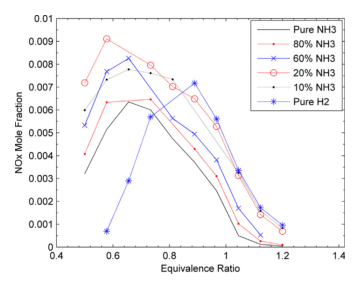
\includegraphics[width=0.7\textwidth]{./pictures/NOxemissions.png}
  \caption{The effect of premixing conditions and fuel-air equivalence ratio on $NO_x$ production when $NH_3/H_2$ mixtures are burned \cite{Nozari2015}} \label{fig:NOxemissions}
  \end{figure}
\subsection{The Turbine Model}
MATLAB was used to model the turbine in a modular approach, where each component was modelled using a separate function. The initial conditions were that the compressor would take in ambient air (298K, 101kPa) and that the adiabatic flame temperature should not exceed 1700K. Derivation of governing equations follows that of Ireland (2017) \cite{thermonotes}.

\subsubsection{Cycle Efficiency}
Cycle efficiency $\eta_{cycle}$ represents the amount of work extracted per unit of heat put into the system.
\begin{equation}
\eta_{cycle} = \frac{w_{out} - w_{in}}{q_{in}}
\end{equation}
Where $w_{out}$ is the total amount of work out of the system (from the turbine), $w_{in}$ is the total work put into the system (through the compressor) and $q_{in}$ is the total heat put into the combustion chamber.

\subsubsection{Wobbe Number} 
The Wobbe number is a measure of the energy output of a given fuel. It can used as an indicator describing interchangeability of different fuels to be used in combustors and is defined as follows \cite{website:wobbe}: 
\begin{equation}
W_B = \frac{LCV}{\sqrt{G_S}}
\end{equation}
Where LCV is the lower calorific value of the fuel ($MJ kg^{-1}$), $G_S$ is the specific gravity of the fuel compared to air. The $NH_3/H_2$ mixture was calculated to have a Wobbe number of 49.1MPa, which is very close to the Wobbe number or propane-air of 50.9MPa \cite{website:wobbe}, and well within the Wobbe variation limits of a typical 90MW gas turbine of $\pm 30\%$ \cite{PDF:GE} indicating that it should burn as propane would in the combustor. 

\subsubsection{Pressure Ratio} 
The pressure ratio of a gas turbine determines cycle temperatures and therefore work input and outputs. Variation in net cycle efficiency was calculated and plotted against a pressure ratio from 1 to 35. It can be compared to the joule cycle efficiency, which represents the maximum efficiency that can be extracted for a given pressure ratio. The specific work input, work output and net work output were also plotted with different pressure ratios. A pressure ratio of 21 was chosen as this results in the maximum efficiency as illustrated in figure \ref{fig:efficiencysimple}.
 \begin{figure} [h]
\centering
\begin{subfigure}{.7\textwidth}
\centering
 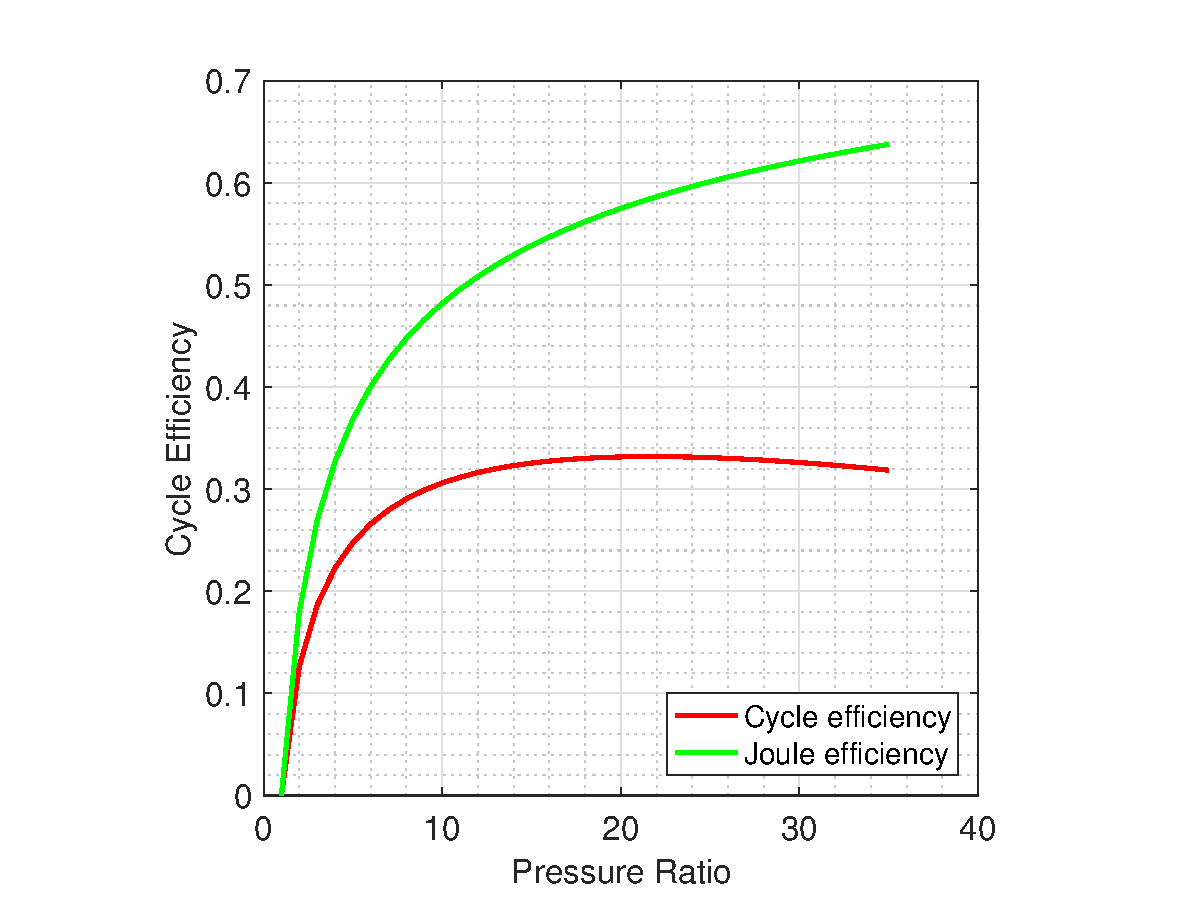
\includegraphics[width=0.9\linewidth]{./pictures/efficiencysimple.eps}
  \label{fig:efficiencysimple}
\end{subfigure}
\begin{subfigure}{.7\textwidth}
 \centering
 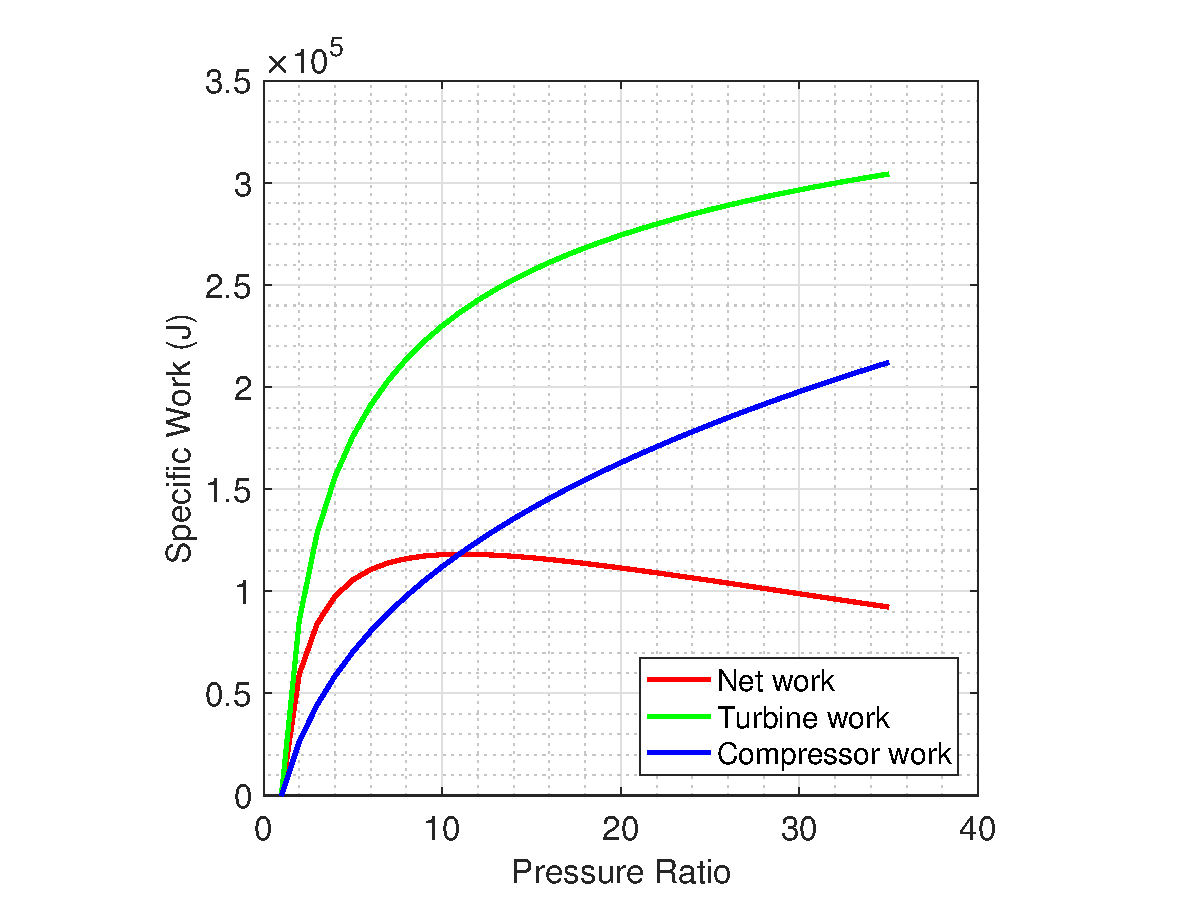
\includegraphics[width=0.9\linewidth]{./pictures/network.eps}
 \label{fig:sub2}
\end{subfigure}
\caption{(a) The actual (red) and joule (green) cycle efficiency across different pressure ratios and (b) the turbine specific work output (green), the net specific work output (red) and the compressor specific work input (blue).}
\label{fig:efficiencysimple}
\end{figure} 

\subsubsection{Compressor} \label{ssec:compressor} %negligible change in velocity and height, SFEE
Both centrifugal and axial flow compressors were considered for the plant, but the axial flow compressor was chosen in the end as its high efficiency and flow rate makes it more suitable for the large scale of the plant. The compressor was modelled as adiabatic and isentropic ($Pv^{\gamma} = k$). The air was modelled as a perfect gas ($Pv = RT$), such that:
\begin{equation}
\frac{T_{2s}}{T_1} = \frac{P_2}{P_1}^{\frac{\gamma-1}{\gamma}}
\end{equation}
$T_{1}$ and $T_{2s}$ are the inlet temperature and the isentropic outlet temperatures respectively ($K$), $P_1$ and $P_2$ are the pressures at the inlet and outlet of the compressor respectively ($kPa$).

Using the definition of compressor isentropic efficiency $\eta_c = {h_{2s} - h_1}/{h_2 - h_1} $, the compressor work in is therefore:
\begin{equation}
W_{c} = \frac {\dot{M}_a \tilde{C}_P}{\eta_c} (T_{2s} - T_1)
\end{equation}
Where $\dot{M}_a$ is the molar flow rate of air ($kmols^{-1}$) and $\tilde{C}_P$ is the molar specific heat capacity at a constant pressure of air ($kJkmol^{-1}K^{-1}$). Using a pressure ratio of 21, an isentropic efficiency of 0.85 and taking the input air at ambient conditions, the compressor outlet temperature was calculated to be 757.1K.  

\subsubsection{Combustor} 
The combustion chamber can be assumed to be adiabatic. For complete combustion and no heating losses, the adiabatic flame temperature can be calculated using:
\begin{equation}
\tilde{C}_{PP} (T_{2P} - T_0) = \tilde{C}_{PR} (T_{1R} - T_0) - LCV 
\end{equation}
Where $T_{2P}$ and $T_{1R}$ represent the temperatures of the products and reactants (K), $T_0$ represents the reference temperature 288K, $\tilde{C}_{PP}$ and $\tilde{C}_{PR}$ represent the heat capacity at constant pressure of the products ($kJK^{-1}$) and reactants and LCV is the calorific value at a constant pressure of the $H_2/NH_3$ mixture ($kJ/kmol$). The heat capacities were calculated using the rule of mixtures $\tilde{C}_{P, mix} = \sum\nolimits M_i \tilde{C}_{P, i}$ where $M_i$ is the molar fraction of each component. %separate air and fuel 

The heat input $Q_{in}$ to the compressor must also be calculated to be used in efficiency calculations.
\begin{equation} \label{eq:heatequation}
Q_{in} = \dot{m}C_P\Delta T
\end{equation}
Where $\dot{m}$ is the mass flow rate into the combustion chamber, $\tilde{C}_P$ is the average specific heat capacity of the reactants and the products ($kJ kg^{-1} K^{-1}$) and $\Delta T$ is the difference in temperature across the combustion chamber.


\subsubsection{Air-Fuel Equivalence Ratio} 
The Air-fuel equivalence ratio $\lambda$ is defined as the ratio of actual and stoichiometric fuel to oxidiser ratio. It determines the energy released for a combustion reaction as well as exhaust products: \begin{equation}
\lambda = \frac{m_{air}/m_{fuel}}{(m_{air}/m_{fuel})_{stoich}}
\end{equation}
where $m_{air}/m_{fuel}$ is the mole ratio of air to fuel. Variations in $\lambda$ must satisfy the lower and upper flammability limits of 6.5-40\% \cite{LFL}, which correspond to $\lambda$ in the range of 0.447 to 4.77, within these flammability limits the equivalence ratio can be varied to control the combustion temperature.
Taking the flame temperature as the limiting value from section \ref{ssec:NOx}, 1700K and a combustor inlet temperature of 757K, the required equivalence ratio was found to be 2.5 as shown in figure \ref{fig:flametemp}.

\begin{figure} [h]
\centering
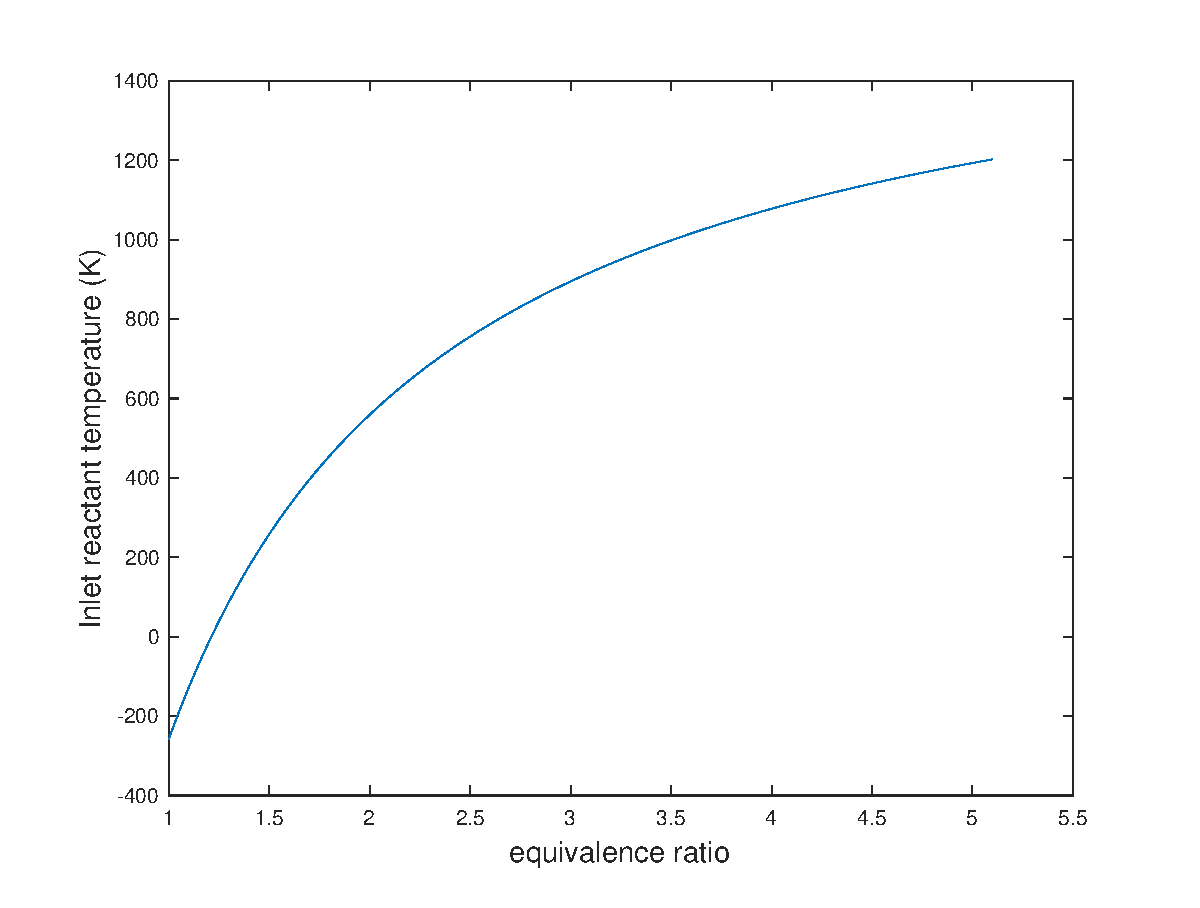
\includegraphics[width=0.7\textwidth]{./pictures/combustor.eps}
  \caption{A chart showing the variation in inlet reactant temperature with equivalence ratio.} \label{fig:flametemp}
  \end{figure} 

\subsubsection{Turbine} \label{ssec:turbine}
The turbine is where power is generated, it is coupled to a generator to provide electricity. An axial-flow turbine will be used for the plant as it more suitable than radial inflow turbines for large flow rates. The turbine model was used to calculate the molar flow rate of pre-cracked ammonia required. The turbine was also modelled as adiabatic and isentropic, and the exhaust as a perfect gas, leading to: 
\begin{equation}
\frac{T_{4s}}{T_{3}} = \frac{P_4}{P_3}^{\frac{\gamma -1}{\gamma}}
\end{equation}
Using the definition of turbine isentropic efficiency $\eta_T = {h_3 - h_4}/{h_3 - h_{4s}}$, the work output is therefore:
\begin{equation}
W_t = \dot{M}_{ex} \tilde{C}_{PP} \eta_t  (T_3 - T_{4s})
\end{equation}
Where $\dot{M}_{ex}$ is the molar flow rate of the exhaust gas ($kg s^{-1}$), $\tilde{C}_{PP}$ is the molar specific heat capacity of the exhaust products ($kJ kg^{-1} K^{-1}$), $\eta_t$ is the turbine isentropic efficiency, $T_3$ and $T_{4s}$ are the temperatures at the turbine inlet and the outlet for an isentropic process respectively ($K$). 

\subsection{Turbine cycle modifications }
The cycle efficiency obtained from the simple cycle turbine was 0.332. In order to increase cycle efficiency, modifications were added to the standard cycle including using a separate power turbine to increase efficiency and using waste oxygen from the electrolyser to decrease the mass flow rate of air. 

\subsubsection{Split-shaft system}
Due to the large size of the plant and the large variation in power output required, it is advantageous to use a split-shaft system which consists of 2 turbines: one is used to transfer work to the compressor, which is called the gas generator. This must be coupled to the compressor and operates at a high pressure. The second is the power turbine used to generate power being supplied to the public, which operates at a lower pressure. This turbine is coupled with the load and must operate at US mains frequency of 60Hz (3600rpm). As the rotational speeds of the two turbines in a split shaft system are independent, the gas generator speed can be varied with the power demand to operate at maximum cycle efficiency. \cite{thermonotes} %show in diagram?

\subsubsubsection{Pressure Ratio}
The efficiency characteristics of the split-shaft system were recalculated as shown in figure \ref{fig:twinefficiency}. It shows that in going from a single shaft to a split-shaft turbine, the maximum efficiency shifts from a pressure ratio of 21 to 17, with a significant increase in efficiency across all pressure ratios. This pressure ratio also gives the maximum specific work output and the minimum ammonia flow rate. A lower combustion pressure has also been linked to fewer $NO_x$ emissions and is safer \cite{junLi}, therefore the pressure ratio of 17 was used in this iteration of the model. 
\begin{figure} [h]
\centering
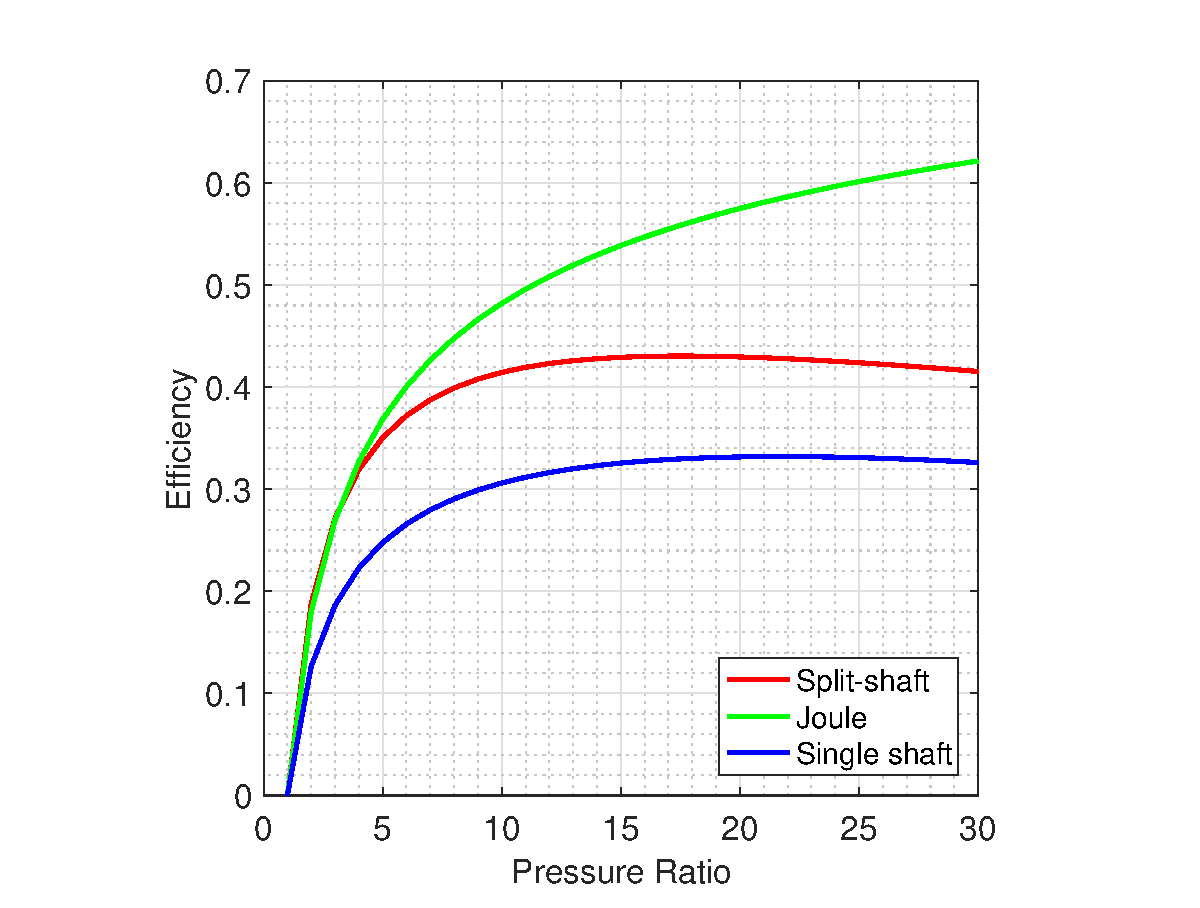
\includegraphics[width=0.7\textwidth]{./pictures/efficiencyPT.eps}
  \caption{Chart showing the change in joule efficiency, split-shaft efficiency and simple cycle efficiency across different pressure ratios} \label{fig:twinefficiency}
  \end{figure}
  
\subsubsubsection{Intermediate Pressure}
Instead of one overall pressure ratio $r_p$, the high and low pressure turbines will have their own pressure ratios $r_{p1}$ and $r_{p2}$ where $r_p = r_{p1} r_{p2}$. The high pressure turbine is used to generate the amount of work that is required by the compressor. This allows us to find the pressure ratio required for the first turbine using the compressor and turbine work equations from sections \ref{ssec:compressor} and \ref{ssec:turbine}:
\begin{equation}
r_{p1} = [1-\frac{C_{p, a} T_1}{\eta_C \eta_T C_{p, p} T_3} (r_p^\frac{\gamma -1}{\gamma}-1)]^{\frac{\gamma}{1-\gamma}}
\end{equation} %uniform Cp across all sections
A pressure ratio of 17.5 was used for the final model, yielding a primary turbine pressure ratio of 2.77 and a secondary pressure ratio of 5.77.

\subsubsubsection{Changes to Model Results}
The effect of using a split-shaft turbine is shown in table \ref{tab:splitshaft}. The split-shaft turbine has greater flow rates but increases efficiency by 10\%, this is a large increase in efficiency, justifying the use of the split-shaft turbine model. 

\begin {table} [h]
\begin{center}
\caption{Salient model results from single shaft and split-shaft turbine configurations} \label{tab:splitshaft} 
\begin{tabular}{ |c|c|c| }
 \hline
  Model Type & Single shaft & Split-shaft\\ 
 \hline
  Efficiency & 0.3320 & 0.4272 \\ 
  \hline
  $NH_3^*$ flow rate (kmol/s) & 0.3246 & 0.6423\\ 
 \hline
  Exhaust Temperature (K) & 909.9 & 917.5\\
  \hline
  Equivalence Ratio & 2.5 & 2.44\\
 \hline
\end{tabular}
\end{center}  
\end {table} %heat or work input?

\subsubsection{Additional Oxygen}
In order to reduce the air flow rate in the compressor, additional oxygen can be added to the combustion chamber. Oxygen enriched combustion is typically used to increase the rate of combustion and increase flame temperature \cite{oxyfuel}. However, the combustor currently already has an excess of air, so the additional oxygen will not increase the flame temperature but will absorb the heat instead. By decreasing the mass flow in the compressor and increasing it in the turbine, there will be a decrease in compressor work and an increase in turbine work, which would increase plant efficiency. 

Both the electrolyser and the air separator produce very pure oxygen as a waste product. However, the oxygen from the air separator is close to ambient pressure and temperature so would have heated significantly to be used. In contrast, the electrolyser produces large amounts of high pressure oxygen, which can be expanded through a turbine before entering the combustion chamber, providing extra work. The results of adding different amounts of oxygen are shown in table \ref{tab:extraox}.

\begin {table} [h]
\begin{center}
\caption{Salient model results from the addition of waste oxygen to combustion chamber} \label{tab:extraox} 
\begin{tabular}{ |c|c|c|c|c|c| }
 \hline
  Oxygen flow rate (kmol/s) & 0 & 0.5 & 1.0 & 1.5 & 2.0\\ 
   \hline
  Equivalence Ratio & 2.44 & 2.23 & 2.03 & 1.82 & 1.62\\
    \hline
  $NH_3^*$ flow rate (kmol/s) & 0.6423 & 0.6425 & 0.6109 & 0.5823 & 0.5562\\ 
    \hline
  Heat in (MW) & 210.5 & 234.8 & 248.2 & 262.9 & 303.3 \\
  \hline
  Efficiency & 0.4274 & 0.387 & 0.3624 & 0.3424 & 0.3073\\ 
 \hline
\end{tabular}
\end{center}  
\end {table} 
The increase in oxygen levels did not have the desired effect on efficiency. Although there was a reduction in air and ammonia flow rate and additional work from the expansion turbine, the temperature of the oxygen coming into the combustion chamber was still too low meaning a greater heat requirement and a decrease in plant efficiency. For this reason the extra oxygen modification was discarded in the final design.


\subsubsection{Heat Engine}
The exhaust gases coming out of the low pressure turbine still hold significant energy due to the high temperature. As this stream cannot be used in the heat exchange network and a combined heat and power system would require a combined cycle turbine, it was decided to run it through a simple heat engine, which converts heat into work. Equation \ref{eq:heatequation} can be used to describe the heat recovered from the engine. The efficiency of a heat engine $\eta_E$ is \cite{thermonotes}:
\begin{equation}
\eta_E = (1 - \frac{T_C}{T_H}) \eta_{rel} 
\end{equation}
Where $T_C$ and $T_H$ are the cold and hot temperatures respectively (K) and the bracketed term represents the Carnot, or maximum possible efficiency for the temperature range $T_H - T_C$ and $\eta_{rel}$ is the actual engine efficiency relative to the Carnot efficiency. Using a relative efficiency of 0.8, the heat engine will output 0.724MW at full load, meaning that the power output required is reduced to 89.3MW leading to an increase in efficiency as shown in table \ref{tab:heatengine}. This justified the use of the heat engine so it was kept for the final design.

\begin {table} [h]
\begin{center}
\caption{Salient model results from the addition of a heat pump to the system} \label{tab:heatengine} 
\begin{tabular}{ |c|c|c| }
 \hline
  Model Type & No Engine & Engine\\ 
  \hline
  $NH_3^*$ flow rate (kmol/s) & 0.6423 & 0.6257\\ 
 \hline
  Heat in (MW) & 211& 207\\
  \hline
  Efficiency & 0.4272 & 0.4353\\
 \hline
\end{tabular}
\end{center}  
\end {table}

\pagebreak
\subsection{Turbine System Overview}
The overall turbine diagram is shown in figure \ref{fig:turbinediagram}. Stream and power data are shown in tables \ref{tab:streamdata} and \ref{tab:powerdata}.

\begin{figure} [h]
\centering
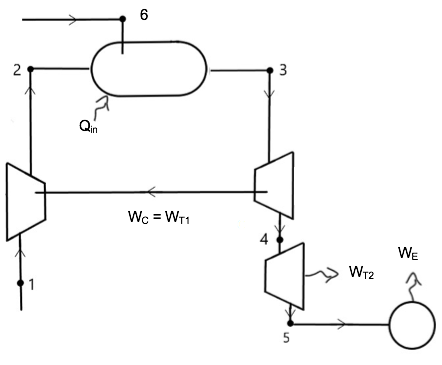
\includegraphics[width=0.58\textwidth]{./pictures/plantdiagram.png}
  \caption{The turbine diagram, showing all streams, work inputs, outputs and heat inputs} \label{fig:turbinediagram}
  \end{figure}
  
\begin {table} [h]
\begin{center}
\caption{Thermodynamic and composition data for all streams of a single turbine operating at full capacity} \label{tab:streamdata}
\begin{tabular}{ |c|c|c|c|c|c|c|c|c|c| }
 \hline
  \multirow{2}{*}{State}  & \multicolumn{7}{|c|}{Molar flow rate (kmol/s)} & \multirow{2}{*}{Temperature (K)} & \multirow{2}{*}{Pressure (kPa)}\\ 
 \cline{2-8}
  & $O_2$ & $N_2^*$ & $N_2$ & $H_2O$ & $NH_3$ & $H_2$ & $Total$  & &\\ 
  \hline
  1 &  \multirow{2}{*}{1.175} & \multirow{2}{*}{4.422} & \multirow{2}{*}{-} & \multirow{2}{*}{-} & \multirow{2}{*}{-} & \multirow{2}{*}{-} & \multirow{2}{*}{5.597} & 298 & 101\\ 
 \cline{1-1} \cline{9-10}
  2  & & & & & & & & 722 & 1621\\
  \hline
  3  & \multirow{4}{*}{0.694} & \multirow{4}{*}{4.422} & \multirow{4}{*}{0.321} & \multirow{4}{*}{0.963} & \multirow{4}{*}{-} & \multirow{4}{*}{-} & \multirow{4}{*}{6.400} & 1700 & 1621\\
  \cline{1-1} \cline{9-10}
  4  & & & & & & & & 1356  & 0584\\
  \cline{1-1} \cline{9-10}
  5  & & & & & & & & 928.8 & 101\\
 \hline
 6  & - & - & 0.122 & - & 0.405& 0.366 & 0.893 & 693 & ? \\ 
 \hline
\end{tabular}
\end{center}  
\end {table} % state 6 pressure

\begin {table} [h]
\begin{center}
\caption{Heat inputs and work outputs of the system} \label{tab:powerdata} 
\begin{tabular}{ |c|c| }
 \hline
  $W_{T1}$ & 80.9MW\\ 
 \hline
  $W_{T2}$ & 89.3MW\\
  \hline
  $W_E$ & 723.6kW\\
 \hline
 $Q_{in}$ & 210.5MW\\
 \hline
 Overall Efficiency & 0.6423\\ 
 \hline
\end{tabular}
\end{center}  
\end {table}

\pagebreak
\subsection{Turbine Control}
Variations in power demand of Maui would lead to different power demands from the gas turbine. A complex control system would need to be used to operate the turbine. A typical control system would have 3 controllers for temperature, acceleration and speed, which pass through a low value select as shown in figure \ref{fig:turbinecont}. However, it was shown by Balagamuran \cite{balagamuran} that temperature and acceleration are rarely selected so can be neglected. A simplified speed controller can be used instead. The structure of the closed loop transfer function with negative feedback is shown below in figure \ref{fig:control}

\begin{figure} [h]
\centering
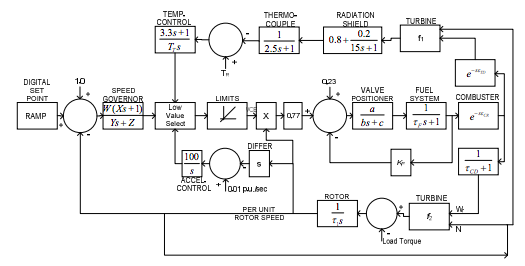
\includegraphics[width=0.85\textwidth]{./pictures/turbinecont.png}
  \caption{The full transfer function of a turbine with temperature, acceleration and speed control \cite{balagamuran}} \label{fig:turbinecont}
  \end{figure}
  
\begin{figure} [h]
\centering
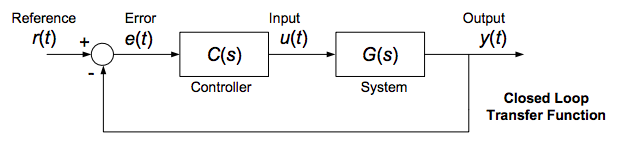
\includegraphics[width=0.7\textwidth]{./pictures/controlsystem.png}
  \caption{A basic control system \cite{A2notes}} \label{fig:control}
  \end{figure}
\subsection{PID Control}

The controller used C(s) will be a saturation limited anti-windup Proportional-Integral-Derivative (PID) controller. PID controllers respond to the error signal itself, in addition to the derivative and the integral of the error signal so that the rise time, settling time and peak overshoot can be controlled by adjusting the variables $P$, $I$, $D$ and $N$ that make up the coefficients of each term. Due to the integral term, PID controllers also have zero steady state error. The transfer function of the PID controller used in Simulink is shown below:
\begin{equation}
P + I\frac{1}{s} + D\frac{N}{1+N\frac{1}{s}}
\end{equation}

\subsubsection{Turbine Transfer Function}
The turbine transfer function G(s), adapted from Balagamuran \cite{balagamuran} consists of several different elements:
\\\textbf{Fuel system:} The fuel system applies the signal from the PID controller $u(t)$ to the active fuel control range, which excludes what is below the minimum load that is required to keep the turbine running under no load conditions and was calculated to be 45\%. This is used to find the fuel flow rate required $\dot{m}_f$. The fuel valve is adjusted accordingly.
\begin{equation}
\dot{m}_f = \frac{1}{0.4s + 1} \frac{1}{0.05 + 1} (0.55u(t) + 0.45)
\end{equation}
\\\textbf{Turbine torque:} Turbine torque is approximated as a linear function of fuel flow rate $\dot{m}_f$ and rotor speed $N$.
\begin{equation}
T = 1.3(\dot{m}_f - 0.45) + 0.5(1 - N)
\end{equation}
\textbf{Rotor}: The rotor system is used to convert the torque signal to a rotor speed using the rotor time constant, which was found to be 20s from turbines of similar size.
\begin{equation}
N = (Turbine \ Torque - Load \ Torque)\frac{1}{20s}
\end{equation}

 \begin{landscape}
\subsubsection{The Control Problem}
The closed loop transfer function was built in Simulink as shown in figure \ref{fig:controlsimulink}. The problem being modelled was a  small step change in load demand of an operating turbine so that start up and shutdown effects are neglected. 
\begin{figure} [h]
\centering
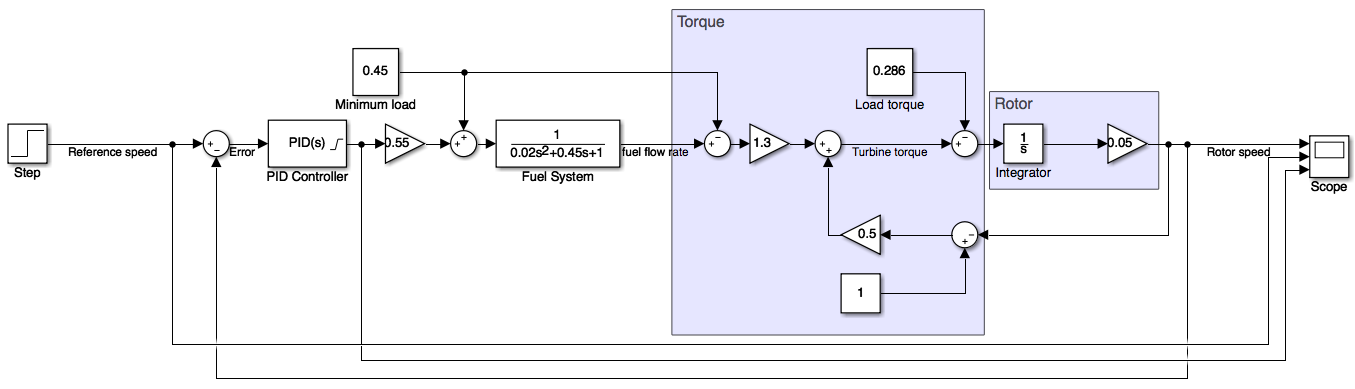
\includegraphics[width=1\textwidth]{./pictures/controlsimulink.png}
 \caption{The control system modelled in Simulink.} \label{fig:controlsimulink} 
 \end{figure}
 The PID tuner built into Simulink was used to adjust the PID parameters to build a closed loop stable system that would achieve the fastest rise time without exceeding a 10\% maximum peak overshoot for step responses over 1MW. A step response was chosen because the turbine is mostly used for sharp rises in power demand, which resembles a step response. Overshoots in step responses less that 1MW were allowed to exceed 10\% as the effect of the overshoot would be very small compared to the power output. The resulting model parameters and results across different sized step inputs are shown in tables \ref{tab:PID} and \ref{tab:controlresults}. The response of the rotor speed, reference speed and PID signal for the 5MW test are also shown in figure \ref{fig:scope}. 
 \end{landscape}

 \begin {table} [h]
\begin{center}
\caption{Parameters of the PID controller derived from Simulinks PID tuner} \label{tab:PID} 
\begin{tabular}{ |c|c| }
 \hline
  P & 1.0502\\ 
 \hline
  I & 0.04338\\ 
  \hline
  D & 1.172\\ 
 \hline
 N & 0.2379\\
 \hline
\end{tabular}
\end{center}  
\end {table}


 \begin {table} [h]
\begin{center}
\caption{Results of the closed loop control system for different step inputs} \label{tab:controlresults} 
\begin{tabular}{ |c|c|c|c|c|}
 \hline
 Size of step input (MW) & 0.5 & 1 & 5 & 10\\
 \hline
  Rise time (s) & \multicolumn{4}{|c|}{38.4}\\ 
 \hline
  Settling time (s) & \multicolumn{4}{|c|}{129}\\ 
  \hline
  Overshoot & 15.6\% & 9.2\% & 5.7\% & 5.3\%\\ 
  \hline
  Peak time (s) & 58.8 & 69.5 & 81.5 & 83.2 \\
 \hline
 Closed loop stability & \multicolumn{4}{|c|}{Stable}\\
 \hline
\end{tabular}
\end{center}  
\end {table}

The model results show a stable rise in power output for all cases, with peak overshoot increasing in magnitude with a smaller step input and occuring earlier.


\begin{figure} [h]
\centering
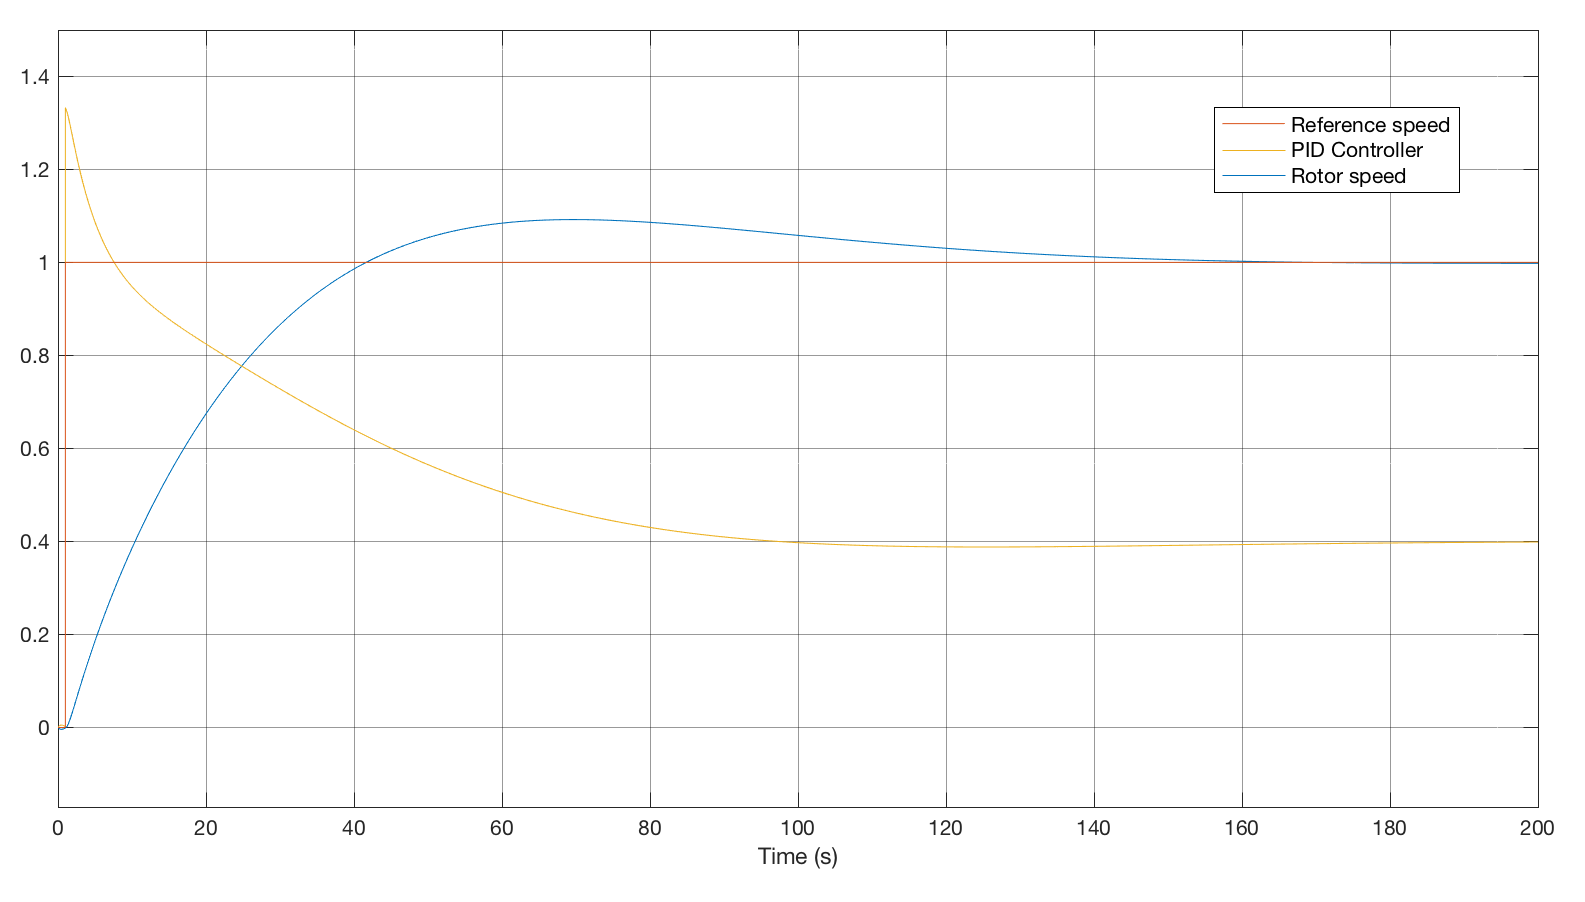
\includegraphics[width=0.9\textwidth]{./pictures/scope.eps}
  \caption{The 1MW step response of rotor speed, reference speed and PID signal} \label{fig:scope}
  \end{figure}

\subsection{Safety \& Risk}
The running of a large gas turbine has many associated risks; A safety and risk analysis was carried out for the gas turbine using a hazard and operability (HAZOP) study. This is to identify all potential hazards associated with the gas turbine coming from deviation to intended operation procedure. Causes and methods to mitigate these risks are split by turbine part and are outlined in table \ref{tab:HAZOP}.

\singlespacing
\begin{longtable}{|L|N |J |M|} 
 \caption{HAZOP study of the gas turbine} \label{tab:HAZOP} \\
    \hline
   Deviation & Cause & Consequences & Action\\
    \hline
    \multicolumn{4}{| c |}{\textbf{Compressor}}\\ 
   \hline
   \multirow{2}{*}{Less air flow} & Blocked air flow valve & Compressor stall - no pressure rise & Continued monitoring of inlet air flow, shut down compressor if no pressure rise\\
   \cline{2-4}
   & Burst pipe & Build up of pressure in pipe, compressor stall & Pressure relief valve in pipe\\
   \hline
   More air flow & Broken air flow valve & Combustion conditions are too lean, ammonia released as exhaust & Continued monitoring of inlet air flow, shut down compressor if there is too much air\\
   \hline
   No air flow & Blocked air flow valve & Compressor stall, build up of pressure in pipe & Continued monitoring of inlet air flow, Pressure relief valve in pipe\\
   Contaminated air flow & Impurities at the air inlet & large impurities can affect reaction, debris can damage machinery & Monitor the composition of the air at the compressor inlet, put plant in an area with clean air, filter out large debris\\
 \hline
 higher temperature & Temperature fluctuations during the year & Combustion temperature is hotter leading to greater $NO_x$, damage to combustion vessel & Monitor combustion temperature and adjust air flow rate accordingly\\
 \hline
    \multicolumn{4}{|c|}{\textbf{Combustor}}\\ 
   \hline
  More fuel flow & Broken fuel valve & Increased combustion temperature, depletion of ammonia reserves & Continued monitoring of combustion chamber temperature, shut down if it exceeds 1800K\\
  \hline
  \multirow{3}{*}{Less fuel flow} & Blocked fuel valve & Mixture may be too lean to burn, ammonia released as exhaust, stored ammonia supply affected, pressure build up in pipe & Continued monitoring of fuel flow, shut down if no combustion, pressure relief valve in pipe\\
   \cline{2-4}
   & Burst Pipe & Ammonia leaks to plant & Ammonia sensor nearby, evacuation at dangerous levels\\
  \cline{2-4}
   & Insufficient ammonia store & No combustion & Continued monitoring of ammonia levels in storage, increase production if it is too low\\
  \hline
  No fuel flow & Blocked fuel valve, insufficient ammonia store & No combustion, no power generated & Continued monitoring of fuel flow, shut down if no combustion, pressure relief valve in pipe\\
  \hline
  Higher temperature & Greater dissociation achieved by pre-cracker & Greater $NO_x$ emissions, damage to combustion vessel & Continued monitoring of combustion chamber temperature, shut down if it exceeds 1800K\\
  \hline
  Lower temperature & Lower input temperature, less dissociation of ammonia, no combustion & Less power generated in turbine & Continued monitoring of combustion chamber temperature, shut down if no combustion\\
  \hline
  Higher pressure & Greater rate of combustion, greater fuel/air flow & Damage to combustion chamber & Pressure sensors in combustion chamber, shut down if pressure exceeds 175kPa\\
  \hline
    \multicolumn{4}{|c|}{\textbf{Turbine}}\\ 
   \hline 
   Higher temperature & Greater dissociation achieved by pre-cracker & Damage caused to turbine machinery & Continued monitoring of combustion chamber temperature, shut down if it exceeds 1800K\\
   \hline
     \multicolumn{4}{|c|}{\textbf{Overall}}\\ 
     \hline
   Other than: system shuts down & no fuel, compressor stall, turbine fault & No power generated & Regular maintenance checks \\
 \hline
 \end{longtable}
\doublespacing

\subsection{Costing}
The main costs of the gas turbine are capital and operation and maintenance (O\&M) costs. Capital costs are the costs for building and installing the gas turbine system, operation and maintenance are required to keep the turbine running well throughout its lifetime. From literature, these are calculated as \cite{turbinecost} \cite{boyce}:
\begin{equation}
Capital \ Cost = 3 [Plant \ Output (kW)] x 763.6 [{Plant \ Output (MW)}^{-0.223}] = \$75.6 \ Million
\end{equation} 
\begin{equation}
O \& M \ Cost = 3 x 5.8 [Plant \ Output (MWh)]= \$1.91 \ Million / year
\end{equation} 

\subsection{Conclusions \& Further Work}
The gas turbine is an effective way to generate power during sharp rises in demand. It is cost effective, reliable and the model shows that it is relatively efficient for the amount of time that it is used. If demand should change by large amounts over time, more turbines can also be added or taken away from the plant due to their modular nature.

One of the largest limitations of the model used was its inability to accurately predict the $NO_x$ formation. The literature did not provide sufficient data for this problem but indicates that in addition to temperature, equivalence ratio also has a large effect on $NO_x$ formation in nitrogen based fuels. This should be studied further across different $NH_3/H_2$ mixtures and different equivalence ratios.
%Nozari


\bibliography{turbine}
%./turbine/
\bibliographystyle{unsrt}
%\printbibliography[heading=subbibliography]


\end{document}